%%%%%%%%%%%%%%%%%%%%%%%%%%%%%%%%%%%%%%%%%%%%%%%%%%%%%%%%%%%%%%%%%%%%%%%%%%%%%%%%
% AMS Beamer series / Bologna FC / Template
% Andrea Omicini
% Alma Mater Studiorum - Università di Bologna
% mailto:andrea.omicini@unibo.it
%%%%%%%%%%%%%%%%%%%%%%%%%%%%%%%%%%%%%%%%%%%%%%%%%%%%%%%%%%%%%%%%%%%%%%%%%%%%%%%%
%\documentclass[handout]{beamer}\mode<handout>{\usetheme{default}}
%
\documentclass[presentation, 10pt]{beamer}\mode<presentation>{\usetheme{AMSBolognaFC}}
%\documentclass[handout]{beamer}\mode<handout>{\usetheme{AMSBolognaFC}}
%%%%%%%%%%%%%%%%%%%%%%%%%%%%%%%%%%%%%%%%%%%%%%%%%%%%%%%%%%%%%%%%%%%%%%%%%%%%%%%%

%\usepackage{lmodern}
\usefonttheme{professionalfonts}
\usepackage{arev}
\usepackage{multicol}
\usepackage{wasysym}
\usepackage{amsmath,blkarray}
\usepackage{centernot}
\usepackage{fontawesome}
\usepackage{fancyvrb}
\usepackage[ddmmyyyy]{datetime}
\renewcommand{\dateseparator}{}
%\renewcommand{\thefootnote}{\fnsymbol{footnote}}
\newcommand{\version}{1}
\usepackage{biblatex}
	\makeatletter

\addbibresource{biblio.bib}
%%%%%%%%%%%%%%%%%%%%%%%%%%%%%%%%%%%%%%%%%%%%%%%%%%%%%%%%%%%%%%%%%%%%%%%%%%%%%%%%
\title[Leveraging LLMs in Software Engineering]
{Leveraging Large Language Models in Software Engineering}
%
\subtitle[Techniques, Challenges, and Opportunities]
{Techniques, Challenges, and Opportunities}
%
\author[\sspeaker{Aguzzi}]
{\speaker{Gianluca Aguzzi} \href{mailto:gianluca.aguzzi@unibo.it}{gianluca.aguzzi@unibo.it}}
%
\institute[DISI, Univ.\ Bologna]
{Dipartimento di Informatica -- Scienza e Ingegneria (DISI)\\\textsc{Alma Mater Studiorum} -- Universit{\`a} di Bologna}
%
\renewcommand{\dateseparator}{/}
\date[\today]{\today}
%
%%%%%%%%%%%%%%%%%%%%%%%%%%%%%%%%%%%%%%%%%%%%%%%%%%%%%%%%%%%%%%%%%%%%%%%%%%%%%%%%
\begin{document}

\nocite{*}
%%%%%%%%%%%%%%%%%%%%%%%%%%%%%%%%%%%%%%%%%%%%%%%%%%%%%%%%%%%%%%%%%%%%%%%%%%%%%%%%

%/////////
\frame{\titlepage}
%/////////
%% print toc
\begin{frame}{Outline}
	\tableofcontents
\end{frame}
%===============================================================================

\section{Introduction to LLMs}
\begin{frame}[plain]
\centering
\huge{
	\textbf{Natural Language Processing} (NLP)
}
\\[1em]
\large{
	{A subfield of artificial intelligence that focuses \emph{understanding}, \emph{interpreting}, and \emph{generating} human language.}
}

\vspace{1em}
\small{
	\textbf{Resources}
	\begin{itemize}
		\item \url{https://github.com/keon/awesome-nlp?tab=readme-ov-file}
		\item \url{https://github.com/brianspiering/awesome-dl4nlp}
		\item \url{https://nlpprogress.com/}
		\item \url{https://www.unibo.it/it/studiare/dottorati-master-specializzazioni-e-altra-formazione/insegnamenti/insegnamento/2023/412644}
	\end{itemize}	
	
}
\end{frame}
\begin{frame}{Natural Language Processing}
	\begin{alertblock}{Goal}
		Identify the structure and meaning of \emph{words}, \emph{phases}, and \emph{sentences} in order to enable computers to understand and generate human language.
	\end{alertblock}
	\begin{exampleblock}{Why?}
		Improve \emph{human-computer} interaction, closing the gap between \emph{human communication} and \emph{computer understanding}.
	\end{exampleblock}
	\begin{alertblock}{Applications \textbf{(all around us)}}
		\begin{multicols}{2}
			\begin{itemize}
				\item \emph{Chatbots}
				\item \emph{Machine Translation}
				\item \emph{Speech Recognition}
				\item \emph{Sentiment Analysis}
				\item \emph{Question Answering}
				\item \emph{Code Generation}
			\end{itemize}
		\end{multicols}
	\end{alertblock}
\end{frame}
\begin{frame}{Natural Language Processing}
    \begin{alertblock}{Challenges}
        \begin{itemize}
            \item \textbf{Ambiguity:} Multiple meanings for words/phrases.
            \item \textbf{Context:} Meaning shifts with context (linguistic, cultural).
            \item \textbf{Syntax:} Sentence structure affects meaning.
            \item \textbf{Sarcasm/Idioms:} Non-literal language interpretation.
        \end{itemize}
    \end{alertblock}
    \begin{exampleblock}{Approaches}
        \begin{itemize}
            \item \textbf{Rule-Based:} Hand-crafted linguistic rules (e.g., \href{https://en.wikipedia.org/wiki/Georgetown-IBM\_experiment}{Georgetown–IBM}).
            \item \textbf{Statistical:} Probabilistic language modelling (e.g., hidden Markov model~\cite{DBLP:journals/coling/Merialdo94}).
            \item \textbf{ML/Deep Learning:} Algorithms learn from data; neural networks model complex patterns (RNN~\cite{DBLP:journals/corr/0001KYS17}, LSTM~\cite{DBLP:journals/neco/HochreiterS97}, GRU~\cite{DBLP:conf/mwscas/DeyS17}).
            \item[\faArrowRight] we will focus on \emph{\textbf{Language Models}}.
        \end{itemize}
    \end{exampleblock}
\end{frame}

\begin{frame}[plain]
	\centering
	\huge{
		What is a \textbf{Language Model}?
	}
	\\[1em]
	\large{
		{A \emph{machine learning} model that aims to predict and generate plausible text.}
	}
\end{frame}
\begin{frame}{Language Models}
	\begin{exampleblock}{Idea}
		text is a sequence of words, and language models learn the \emph{probability} of a word given the previous words.
	\end{exampleblock}
	\begin{exampleblock}{Example}
		\begin{itemize}
			\item \emph{The cat is on the <*>}
			\item \emph{The cat is on the \textbf{mat}.}
			\item \emph{The cat is on the \textbf{table}.}
		\end{itemize}
	\end{exampleblock}
	\begin{alertblock}{Tasks}
		\begin{itemize}
			\item \emph{Prediction:} Given a sequence of words, predict the next word (e.g., autocomplete).
			\item \emph{Classification:} Given a sequence of words, classify the text (e.g., sentiment analysis).
		\end{itemize}
	\end{alertblock}
\end{frame}
\begin{frame}{Language Models -- Phases}
    \begin{enumerate}
        \item \textbf{Tokenization}: Split text into words, phrases, symbols, etc. \\
        \begin{itemize}
			\item \textit{Example:} "Hello, world!" $\rightarrow$ ["Hello", ",", "world", "!"]
		\end{itemize}
        \item \textbf{Embedding}: Convert words into numerical vectors.
        \begin{itemize}
			\item \textit{Example:} "Hello" $\rightarrow$ [0.25, -0.75, 0.5, 1.0]
			\item it is possible to used pretrained embeddings (e.g., Word2Vec,  BERT).
		\end{itemize}
        
        \item \textbf{Modelling}: Learn the probability of a word given the previous words.
        \begin{itemize}
			\item \textit{Example:} P("world" | "Hello,") $\rightarrow$ 0.8
		\end{itemize}
        \item \textbf{Generation/Classification}: Use the model to generate text or classify it. \\
        \begin{itemize}
			\item \textit{Example for Generation:} Input: "The weather is" $\rightarrow$ Output: "sunny." \\
			\item     \textit{Example for Classification:} Input: "This is a spam email." $\rightarrow$ Output: Spam
     
		\end{itemize}
    \end{enumerate}
\textbf{Note:} each NLP solution can use different techniques for each phase.
\end{frame}
\begin{frame}[fragile]{Language Models -- Recurrent Neural Networks}

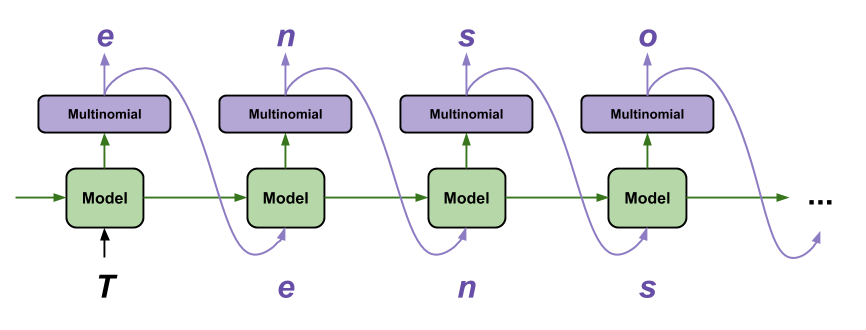
\includegraphics[width=\textwidth]{img/text-generation.png}

\end{frame}

\begin{frame}{Language Models -- Convolutional Networks}

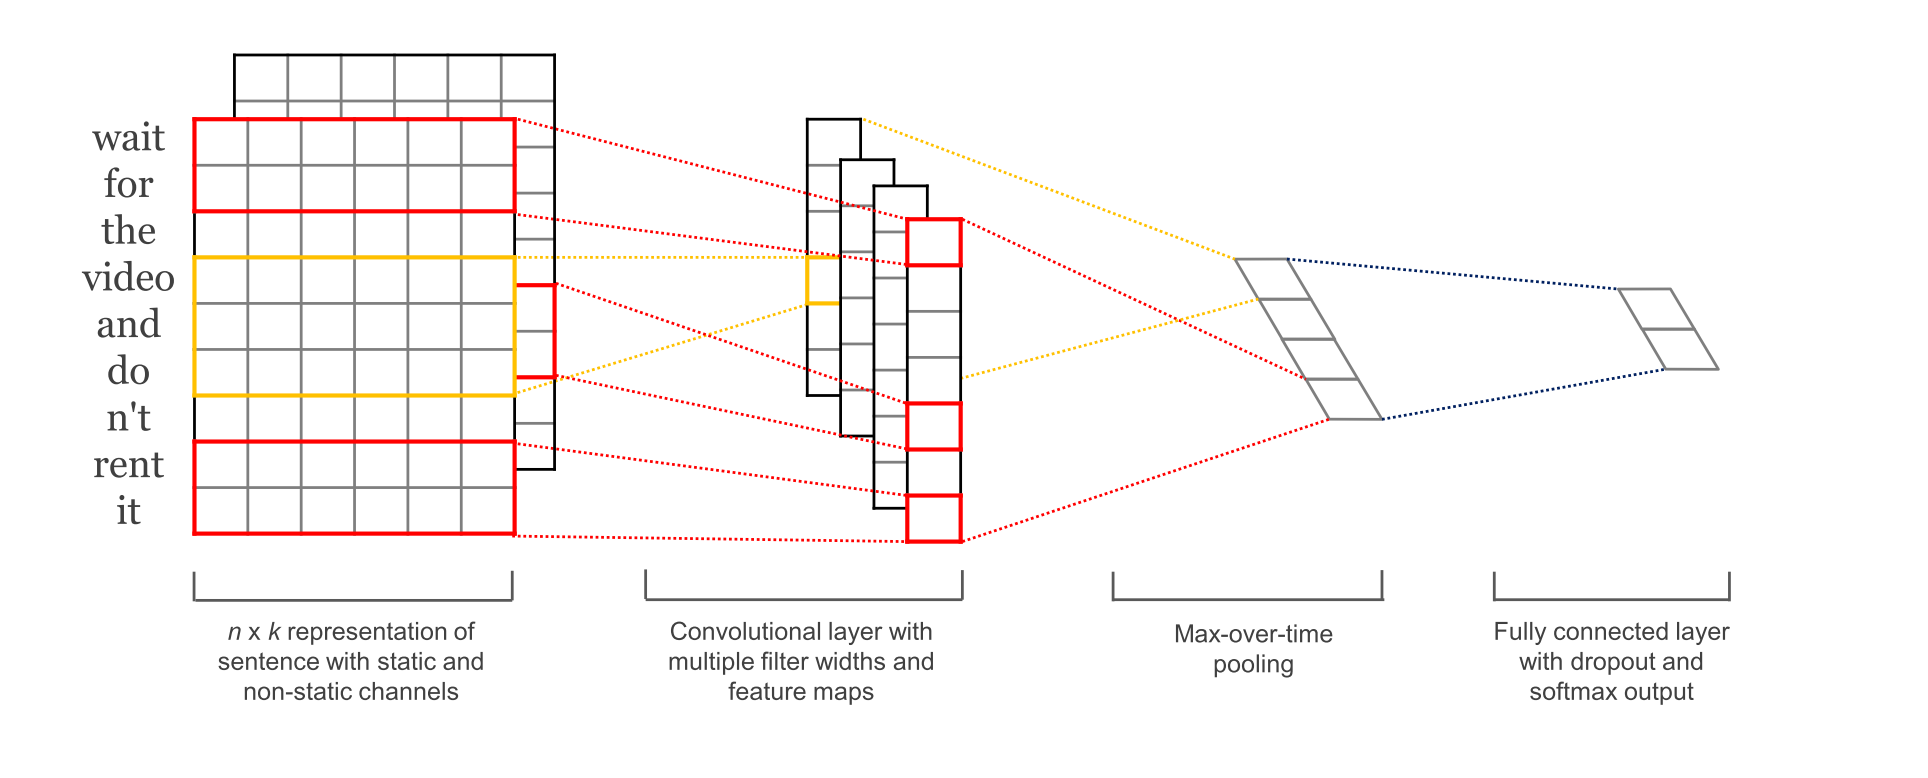
\includegraphics[width=\textwidth]{img/cnn-text.png}

\end{frame}

\begin{frame}{RNN and CNN -- Limitations}
\begin{itemize}
	\item \textbf{RNN:} Long-term dependencies are hard to capture.
	\item \textbf{RNN:} Slow to train; not suitable for large-scale data.
	\item \textbf{CNN:} Fixed-size input; not suitable for variable-length text
	\item \textbf{Both:} Struggle with large-scale data.
	\item \textbf{Solution:} \emph{Multi-head attention}: that is the core of \emph{transformers}.
\end{itemize}
\end{frame}
\begin{frame}{Language Models -- Transformers~\cite{DBLP:conf/nips/VaswaniSPUJGKP17}}
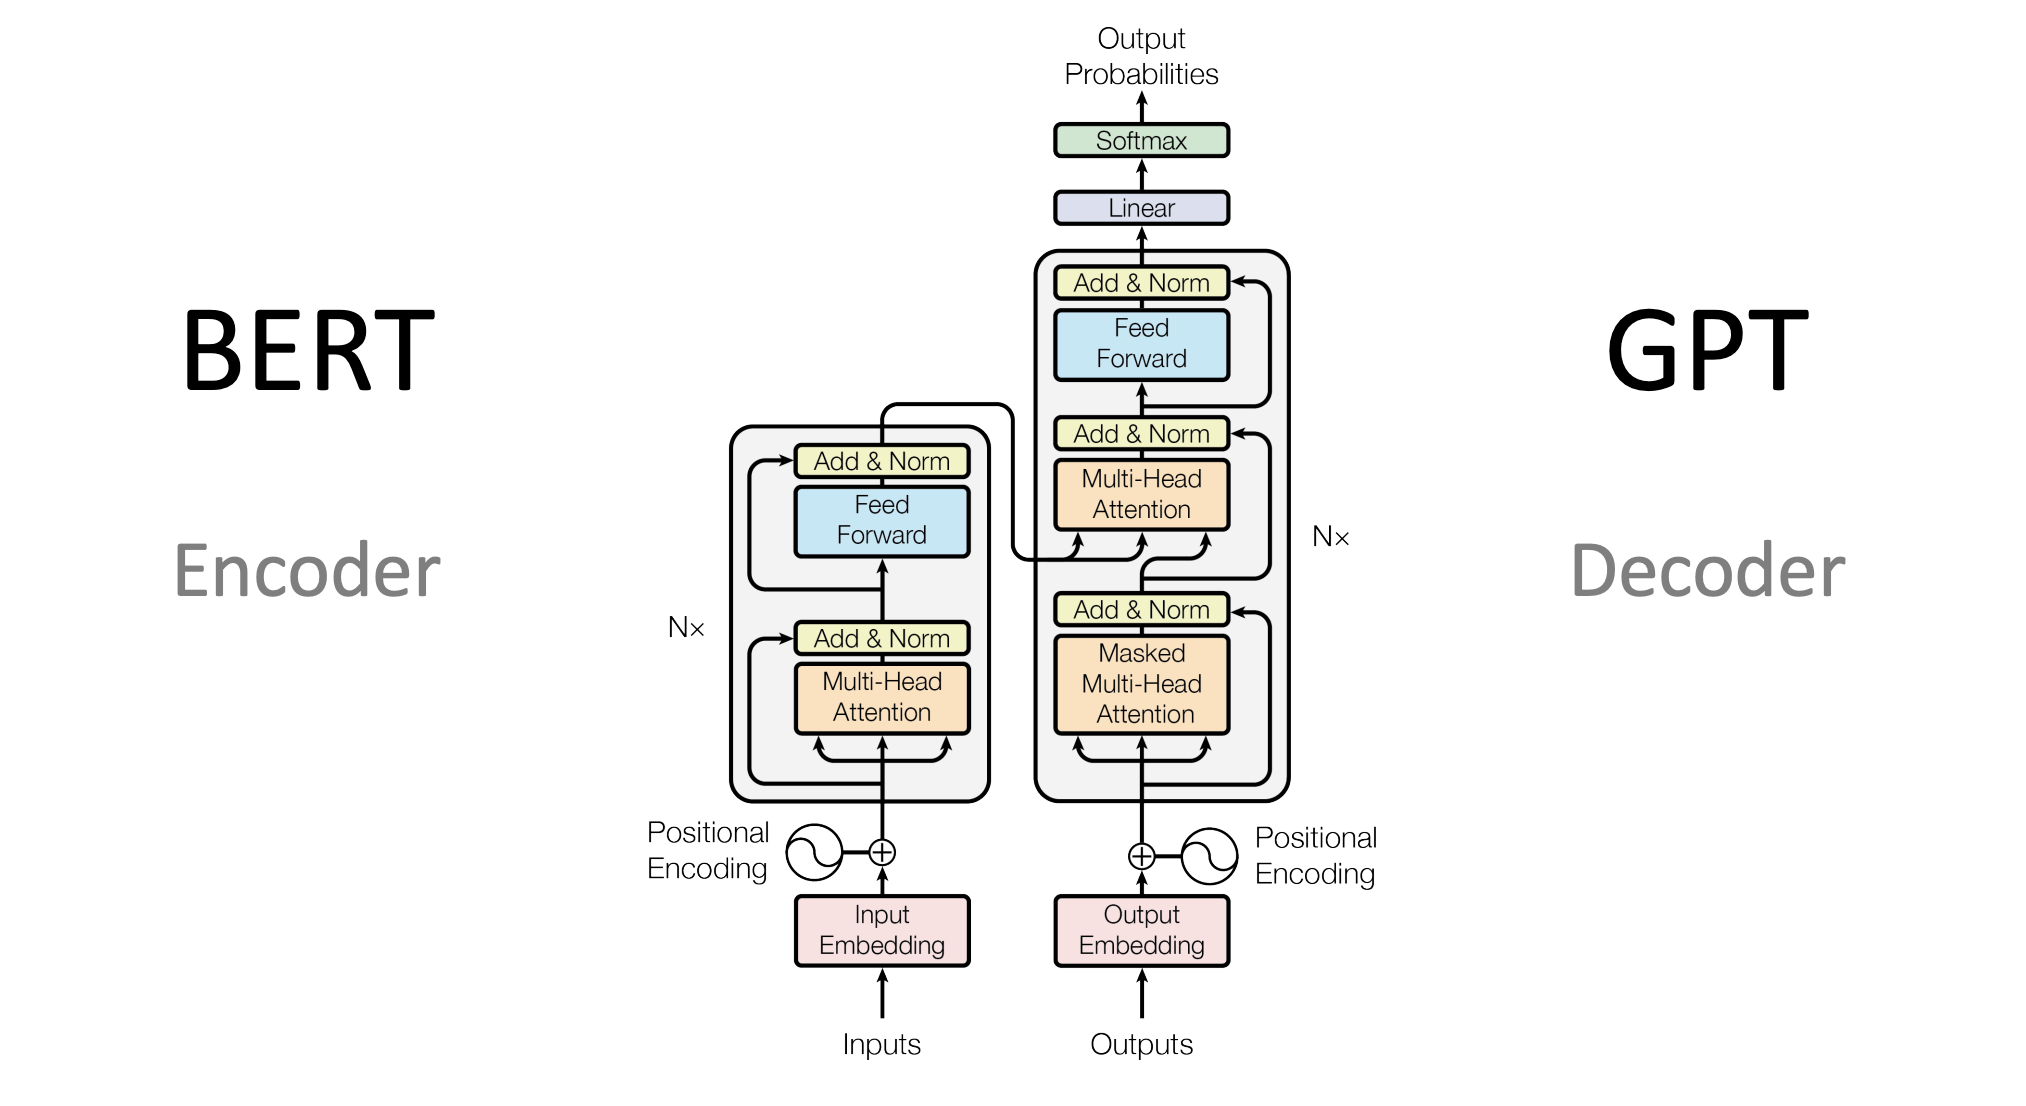
\includegraphics[width=\textwidth]{img/transformers.png}
\centering{
\url{https://www.youtube.com/watch?v=4Bdc55j80l8}
\url{https://www.youtube.com/watch?v=SZorAJ4I-sA}

}
\end{frame}

\begin{frame}[plain]
	\huge{
		\textbf{Large Language Model} (LLM)
	}\\[1em]
	\large{
		{A \emph{language model} with a \emph{large} number of parameters, trained on a \emph{large} corpus of text.}
	}
\end{frame}

\begin{frame}{LLM -- Implementation Strategies}
    \begin{itemize}
        \item \textbf{Transformers} as the foundational architecture, characterized by:
        \begin{itemize}
            \item Long-range context (\emph{Attention})
            \item Efficient large-scale training (\emph{Parallelization})
            \item Model growth (\emph{Scalability})
        \end{itemize}
        \item \textbf{Pretraining:} Involves training the model on a vast corpus of text to learn a wide range of language patterns and structures.
        \item \textbf{Fine-tuning:} Refines the pretrained model for specific tasks, enhancing its applicability and performance on targeted applications.
    \end{itemize}
\end{frame}

\begin{frame}{LLM -- Training Paradigms}
\textbf{The Learning Cake:} An analogy to describe the layered approach in training methodologies.
\begin{itemize}
    \item \textbf{Self-supervised Learning:} Models learn patterns from unlabelled data, reducing the need for expensive annotations. Ideal for initial \emph{understanding} of language structures.
    \item \textbf{Supervised Learning:} Enhances accuracy with labeled data, crucial for tasks requiring specific outcomes like \emph{classification} and \emph{translation}.
    \item \textbf{Reinforcement Learning:} Adapts through trial and error using rewards, fine-tuning decision-making skills in scenarios like \emph{dialogue generation}.
\end{itemize}
\end{frame}
\begin{frame}{LLM -- Paradigm Shift}
	\centering
	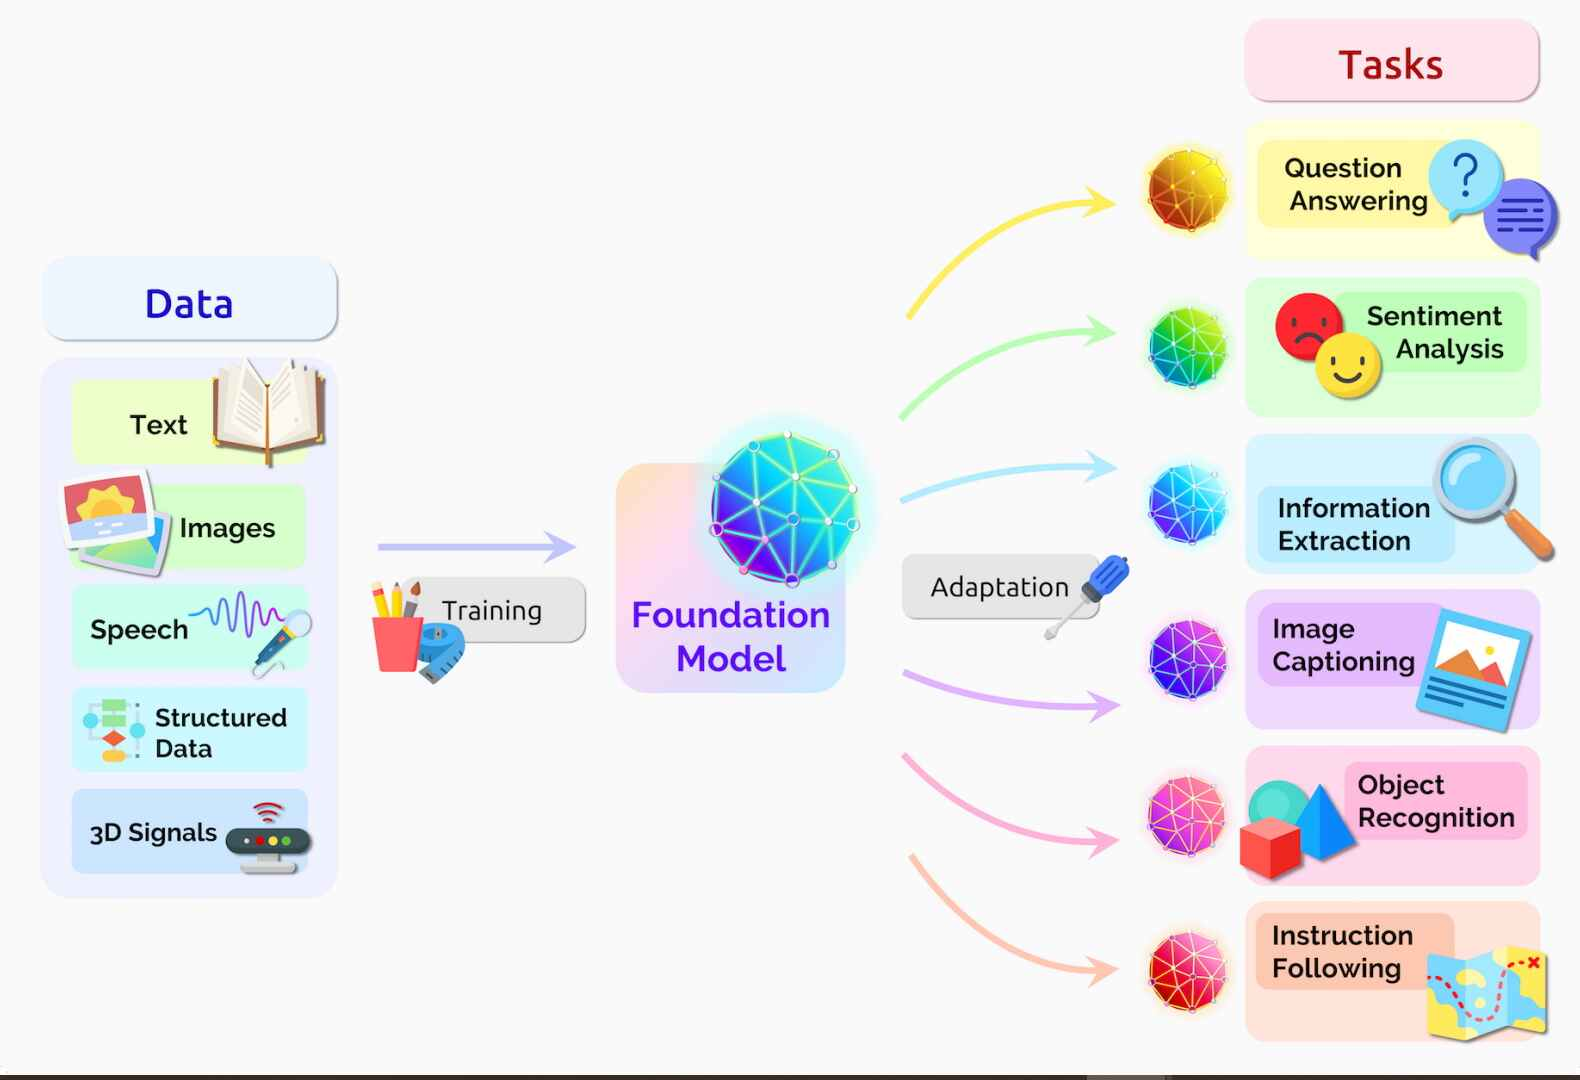
\includegraphics[height=7.5cm]{img/llm-idea.jpg}
\end{frame}
\begin{frame}{LLM -- Scalability}
	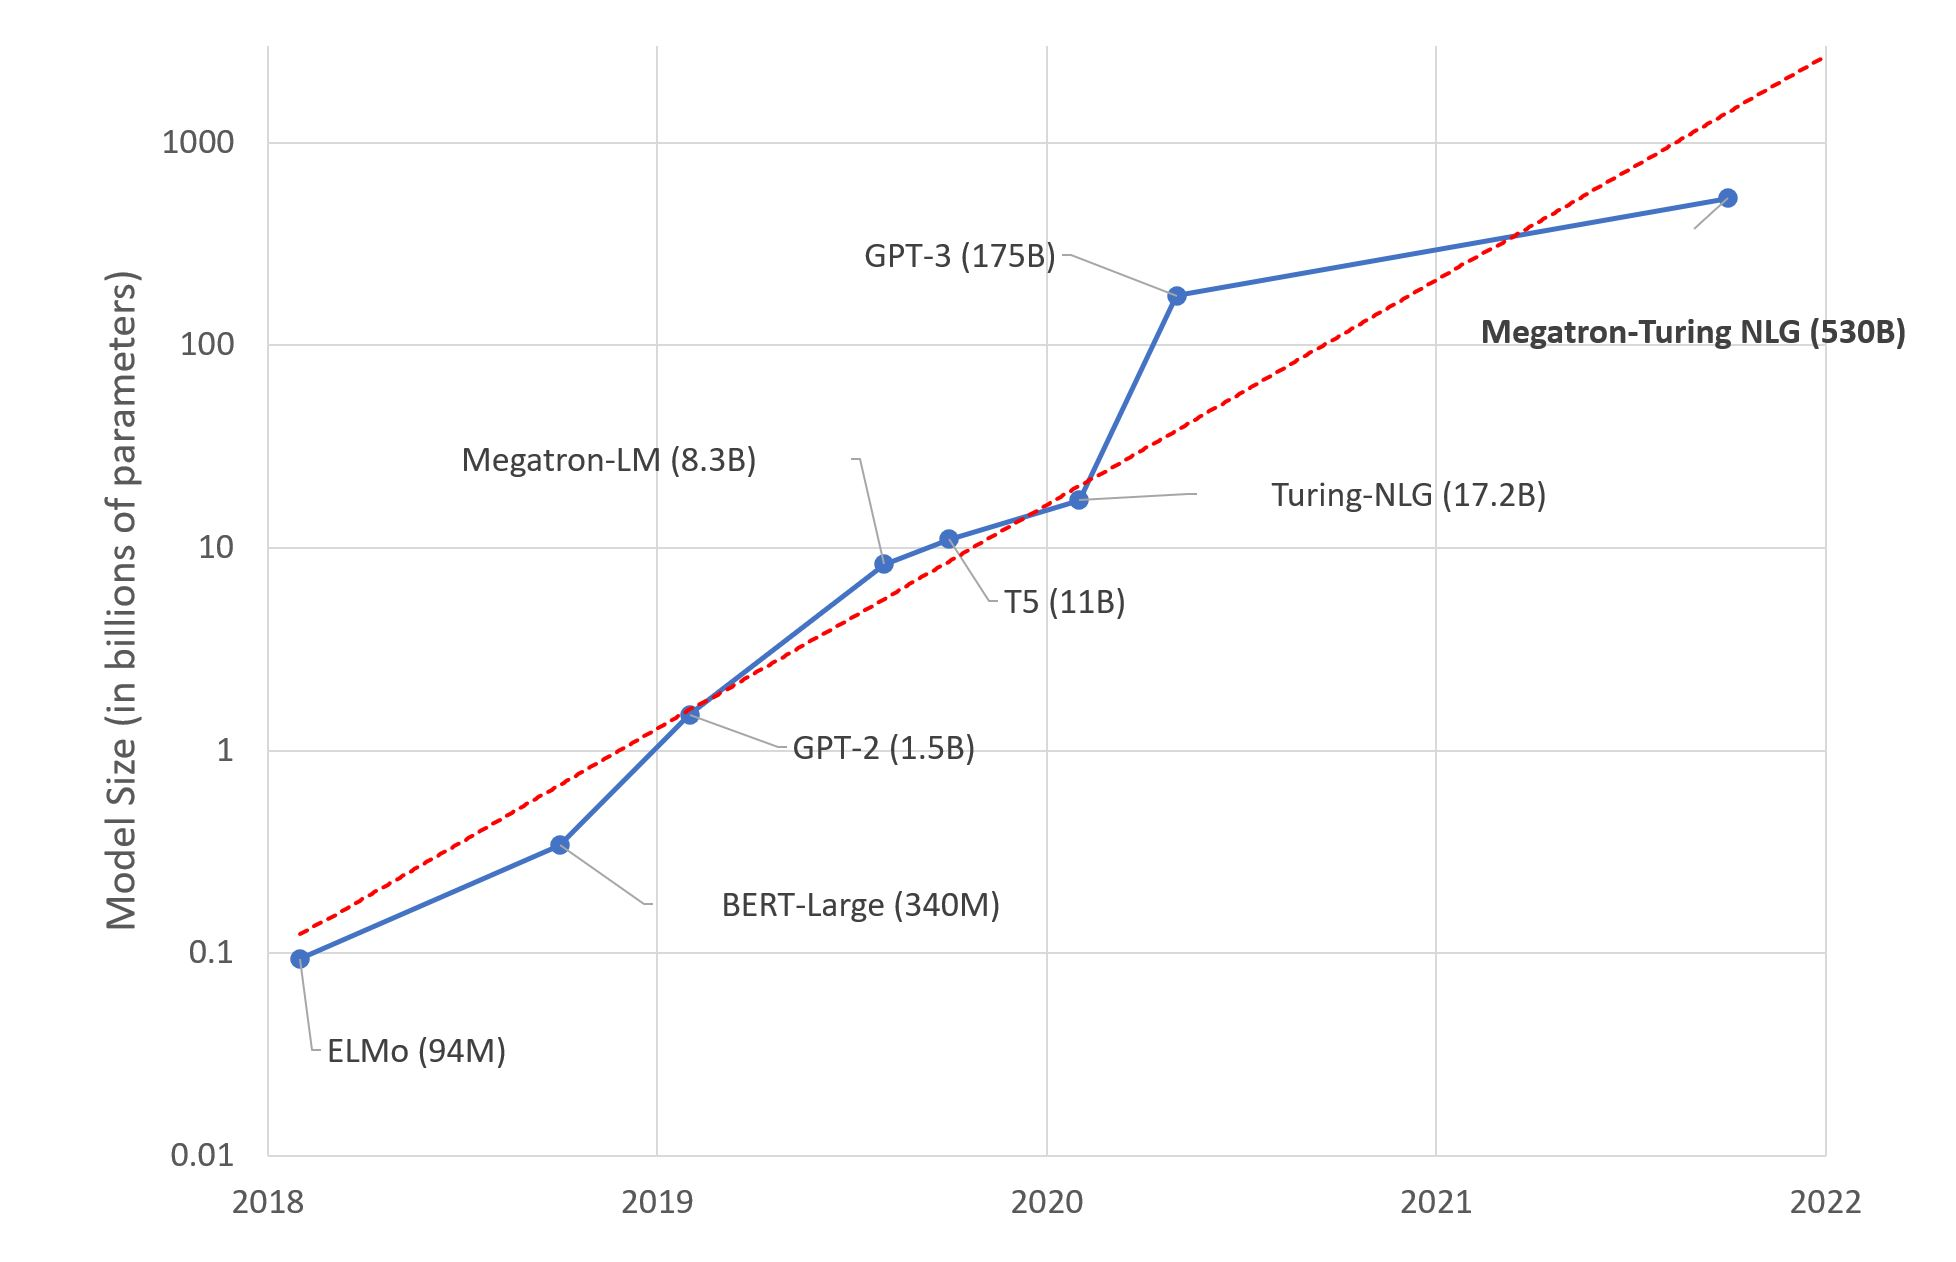
\includegraphics[width=\textwidth]{img/over-year.jpg}
\end{frame}
\begin{frame}{LLM -- Scalability}
	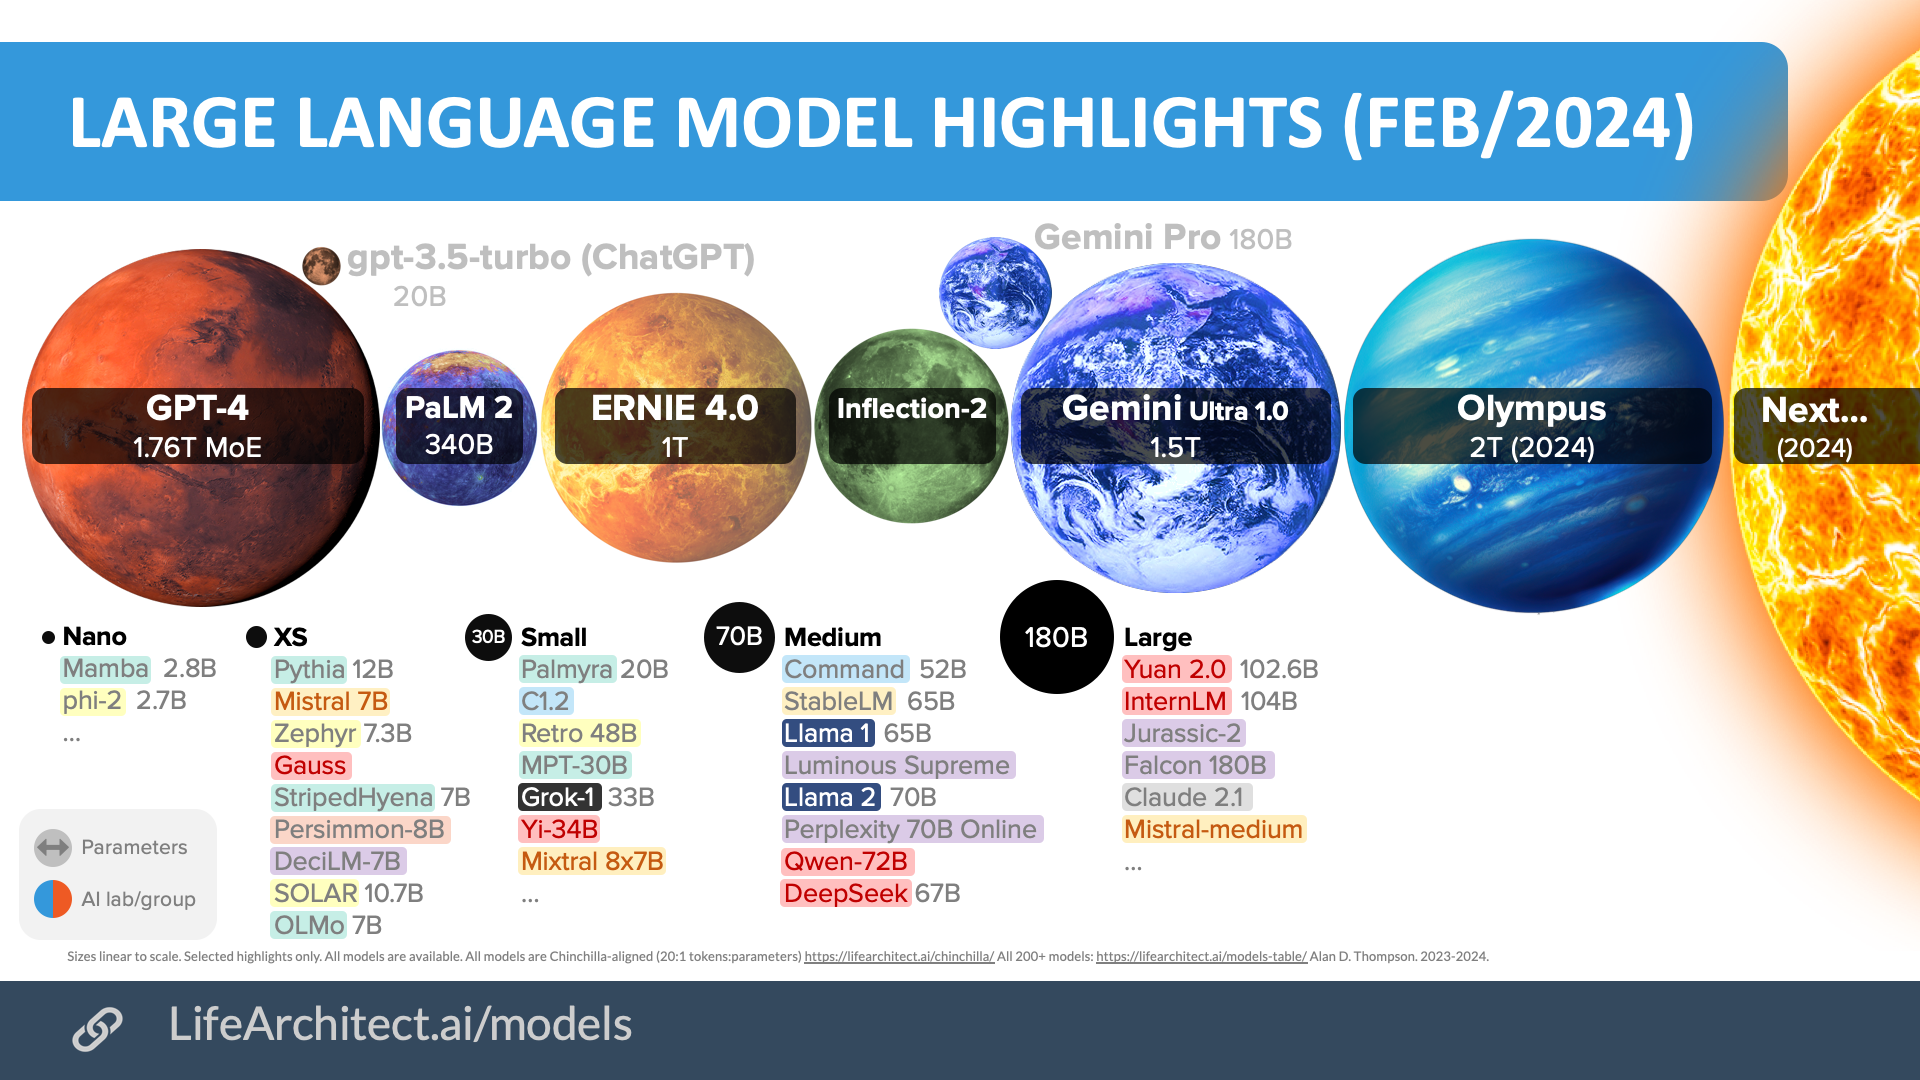
\includegraphics[width=\textwidth]{img/image-size.png}
\end{frame}
\begin{frame}{LLM -- Emergent Properties}
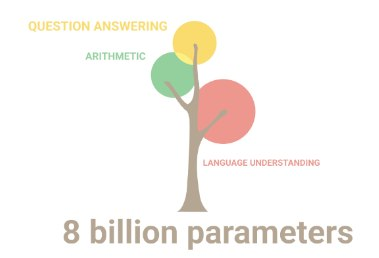
\includegraphics[width=0.35\textwidth]{img/small.jpg}
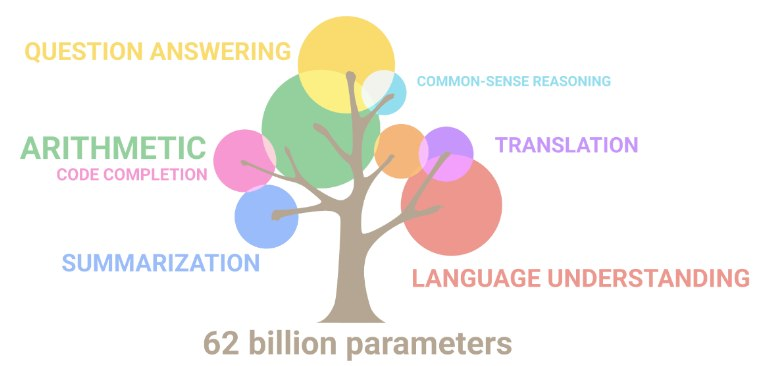
\includegraphics[width=0.55\textwidth]{img/medium.jpg}
\centering
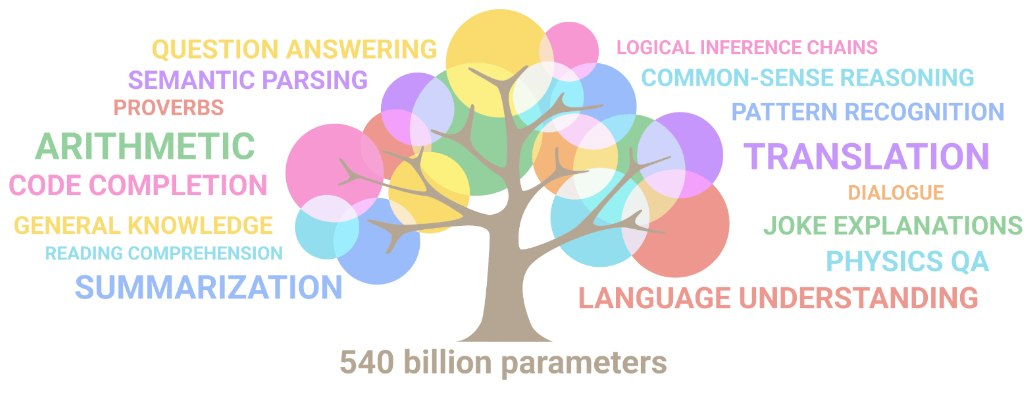
\includegraphics[width=0.8\textwidth]{img/big.jpg}

\end{frame}
\section{Machine Learning for Software Engineering}
\section{LLMs in Software Engineering}

\section{LLMs for Software Testing}

\section{Innovative Solutions for LLMs -- autonomous agent models}
%===============================================================================

%/////////
\frame{\titlepage}
%/////////

%===============================================================================
\section*{\refname}
%===============================================================================

%%%%
\setbeamertemplate{page number in head/foot}{}
%/////////
\begin{frame}[c,noframenumbering, allowframebreaks]{\refname}
%\begin{frame}[t,allowframebreaks,noframenumbering]{\refname}
	\tiny
	\printbibliography
\end{frame}
%/////////

%%%%%%%%%%%%%%%%%%%%%%%%%%%%%%%%%%%%%%%%%%%%%%%%%%%%%%%%%%%%%%%%%%%%%%%%%%%%%%%%
\end{document}
%%%%%%%%%%%%%%%%%%%%%%%%%%%%%%%%%%%%%%%%%%%%%%%%%%%%%%%%%%%%%%%%%%%%%%%%%%%%%%%%
